\documentclass[11pt,oneside]{article}

\usepackage[a4paper,margin=27mm,headheight=15pt]{geometry}
\usepackage[T1]{fontenc}
\usepackage[utf8]{inputenc}
\IfFileExists{libertinus.sty}{\usepackage{libertinus}}{\usepackage{lmodern}}
\usepackage{microtype}
\usepackage{amsmath,amssymb,amsthm,mathtools,mathrsfs}
\usepackage{bm}
\usepackage{booktabs,longtable,array,tabularx}
\usepackage{graphicx}
\usepackage{pgfplots}
\usepackage{xcolor}
\usepackage{enumitem}
\usepackage{fancyhdr}
\usepackage{titlesec}
\usepackage{listings}
\usepackage{xurl}
\usepackage{hyperref}
\usepackage[nameinlink,noabbrev]{cleveref}

\definecolor{linkblue}{RGB}{25,75,135}
\definecolor{shadegray}{RGB}{246,247,249}
\definecolor{rulegray}{RGB}{195,201,208}
\pgfplotsset{compat=1.18}
\hypersetup{
  colorlinks=true,
  linkcolor=linkblue,
  citecolor=linkblue,
  urlcolor=linkblue,
  pdftitle={Nowhere Analyticity of Every Positive Compositional Iterate of the Fabius Function},
  pdfauthor={Research report prepared for the ProveIt Fabius-function corpus},
  pdfsubject={Fabius function, Rvachev up-function, Thue--Morse sequence, Faa di Bruno formula},
  pdfkeywords={Fabius function, nowhere analytic, composition, Rvachev, Thue--Morse, Bell polynomials}
}

\pagestyle{fancy}
\fancyhf{}
\fancyhead[L]{\small Fabius compositional iterates}
\fancyhead[R]{\small\nouppercase{\leftmark}}
\fancyfoot[C]{\thepage}
\renewcommand{\headrulewidth}{0.4pt}

\titleformat{\section}{\Large\bfseries}{\thesection}{0.7em}{}
\titleformat{\subsection}{\large\bfseries}{\thesubsection}{0.7em}{}
\titleformat{\subsubsection}{\normalsize\bfseries}{\thesubsubsection}{0.7em}{}
\setcounter{secnumdepth}{3}
\setcounter{tocdepth}{2}
\setlist[itemize]{leftmargin=2em,itemsep=0.25em,topsep=0.4em}
\setlist[enumerate]{leftmargin=2.3em,itemsep=0.25em,topsep=0.4em}

% Long unbreakable inline mathematics occasionally leaves a line with no legal
% break point.  A small emergency stretch lets TeX loosen such a line rather
% than let it protrude into the margin; it applies only to lines that would
% otherwise be overfull.
\setlength{\emergencystretch}{2em}

\newtheorem{theorem}{Theorem}[section]
\newtheorem{proposition}[theorem]{Proposition}
\newtheorem{lemma}[theorem]{Lemma}
\newtheorem{corollary}[theorem]{Corollary}
\newtheorem{conjecture}[theorem]{Conjecture}
\theoremstyle{definition}
\newtheorem{definition}[theorem]{Definition}
\newtheorem{algorithm}[theorem]{Algorithm}
\newtheorem{example}[theorem]{Example}
\theoremstyle{remark}
\newtheorem{remark}[theorem]{Remark}
\newtheorem{warning}[theorem]{Warning}

\newcommand{\R}{\mathbb R}
\newcommand{\C}{\mathbb C}
\newcommand{\Q}{\mathbb Q}
\newcommand{\N}{\mathbb N}
\newcommand{\Z}{\mathbb Z}
\newcommand{\Up}{\operatorname{up}}
\newcommand{\sinc}{\operatorname{sinc}}
\newcommand{\wt}{\operatorname{wt}_2}
\newcommand{\e}{\mathrm e}
\newcommand{\ii}{\mathrm i}
\newcommand{\dd}{\,\mathrm d}
\newcommand{\Li}{\operatorname{Li}}
\newcommand{\Var}{\operatorname{Var}}
\newcommand{\E}{\mathbb E}
\newcommand{\Prob}{\mathbb P}
\newcommand{\bigO}{\mathcal O}
\newcommand{\smallo}{o}
\newcommand{\supp}{\operatorname{supp}}
\newcommand{\sgn}{\operatorname{sgn}}
\newcommand{\lcm}{\operatorname{lcm}}
\newcommand{\vtwo}{v_2}
\newcommand{\qbinom}[3]{\genfrac{[}{]}{0pt}{}{#1}{#2}_{#3}}
\newcommand{\repo}{\nolinkurl{Analysis/FabiusFunction}}
\newcommand{\lean}[1]{%
  \ifmmode\text{\nolinkurl{#1}}\else\nolinkurl{#1}\fi}
\newcommand{\leanevaltwo}[1]{%
  \nolinkurl{integral_eval}\texttt{\textsubscript{2}}\nolinkurl{#1}}

\newenvironment{proofidea}{\par\smallskip\noindent\textit{Proof architecture.}\ }{\hfill$\square$\par\smallskip}
\newenvironment{boxedremark}{%
  \par\smallskip\noindent\begin{center}\begin{minipage}{0.94\textwidth}%
  \color{black}\hrule\vspace{0.6em}\small
}{%
  \vspace{0.6em}\hrule\end{minipage}\end{center}\smallskip
}

\lstdefinestyle{pseudo}{
  basicstyle=\ttfamily\small,
  backgroundcolor=\color{shadegray},
  frame=single,
  rulecolor=\color{rulegray},
  columns=fullflexible,
  keepspaces=true,
  showstringspaces=false,
  xleftmargin=0.7em,
  xrightmargin=0.7em,
  aboveskip=0.8em,
  belowskip=0.8em
}

% Necessary report-local notation; the shared preamble above is otherwise
% identical to the primary Fabius--Rvachev exposition.
\newcommand{\D}{\mathcal{D}}
\newcommand{\eps}{\varepsilon}
\newcommand{\id}{\operatorname{id}}
\newcommand{\littleo}{o}
\newcommand{\abs}[1]{\left\lvert #1\right\rvert}
\newcommand{\set}[1]{\left\{#1\right\}}
\newcommand{\comp}{\mathbin{\circ}}
\newcommand{\ThetaF}{\Theta}
\newcommand{\half}{\tfrac12}
\newcommand{\statusnote}[1]{%
  \begin{center}
  \fcolorbox{linkblue}{shadegray}{\parbox{0.91\textwidth}{\small #1}}
  \end{center}
}

\title{\bfseries Nowhere Analyticity of Every Positive\\Compositional Iterate of the Fabius Function\\[0.5em]
\large A dyadic-spine proof through Fa\`a di Bruno partitions}
\author{Research report prepared for the ProveIt Fabius-function corpus}
\date{30 August 2026}

\begin{document}
\maketitle

\statusnote{\textbf{Result status.}
The theorem proved here is a new mathematical extension of the repository's formally verified base case.
The proof is self-contained at manuscript level and has received a repository claim-level review, while the supplied floating-point diagnostics are finite-order checks only.  No independent symbolic-verification artifact is supplied, and the theorem has not yet been translated into Lean.
Repository statements explicitly marked as formalized are used only as established input facts; the composition theorem, the weighted partition-defect lemma, and the spine asymptotic are proved in this report.}

\begin{abstract}
Let $F\colon[0,1]\to[0,1]$ be the bounded Fabius function and let
$F^{\comp n}$ denote its $n$-fold compositional iterate.  We prove that, for every
integer $n\geq1$, the smooth function $F^{\comp n}$ is real analytic at no point of
$[0,1]$.  In fact we establish the stronger statement that, for each fixed $n$, the
Taylor series of $F^{\comp n}$ has radius of convergence zero at every point of a
co-countable dense subset of $(0,1)$.

The proof has three ingredients.  First, the exact derivative atlas for the Fabius
function gives
\[
 F^{(m)}(x)=Q_m\Theta(2^m x),\qquad
 Q_m=2^{\binom{m+1}{2}},
\]
where $\Theta$ is the bounded signed global extension whose signs are governed by the
Thue--Morse sequence.  Second, a set-partition form of the Fa\`a di Bruno formula is
split into two extremal chain-rule terms and a genuinely branched remainder.  A new
``dyadic defect''
\[
 D(\pi)=\binom m2-\binom{|\pi|}{2}-\sum_{B\in\pi}\binom{|B|}{2}
\]
shows that the total branched remainder is exponentially smaller than the extremal
terms after normalization by $Q_m$.  Iterating this reduction yields a finite spine
sum indexed by the orbit $x,F(x),\ldots,F^{\comp(n-1)}(x)$.  Third, the orbit dynamics
make the corresponding exponential spine weights strictly unimodal, apart from a
finite tie set, while binary digit transitions force the dominant Thue--Morse amplitude
to remain bounded away from zero along infinitely many derivative orders.  The
resulting derivative lower bound grows like $Q_m$ times an ordinary exponential, far
faster than $m!$, and hence forces zero Taylor radius.

The report also records consequences for inverse iterates and local elementary
representations, gives a reproducible sinc-product computation, and formulates
several concrete research directions involving tie-point cancellation, $q$-Bell
polynomials, Lambert--$W$ endpoint transseries, Legendre expansions, and formalization.
\end{abstract}

\tableofcontents
\newpage

\section{Statement of the problem and the strengthened result}

The bounded Fabius function is the unique smooth increasing bijection
$F\colon[0,1]\to[0,1]$ satisfying
\begin{equation}
  F(0)=0,\qquad F(1-x)=1-F(x),\qquad F'(x)=2F(2x)
  \quad(0\leq x\leq\half),
  \label{eq:basic-F}
\end{equation}
with the usual constant continuation outside the unit interval when derivatives at
endpoints are discussed.  We write
\[
  G_n:=F^{\comp n},\qquad G_0:=\id.
\]
Every $G_n$ is $C^\infty$ because it is a finite composition of smooth functions.
The question is whether composition might suppress the derivative oscillation that
makes $F$ itself nowhere analytic.  The answer is no.

\begin{theorem}[Main theorem]
\label{thm:main}
For every integer $n\geq1$, the compositional iterate $G_n=F^{\comp n}$ is not real
analytic at any point of $[0,1]$.
\end{theorem}

The proof actually gives considerably more.

\begin{theorem}[Co-countable zero-radius set]
\label{thm:strong}
Fix $n\geq1$.  There exists a co-countable dense set $E_n\subset(0,1)$ such that, for
every $x\in E_n$,
\begin{equation}
 \limsup_{m\to\infty}
 \left(\frac{\abs{G_n^{(m)}(x)}}{m!}\right)^{1/m}=+\infty.
 \label{eq:infinite-limsup}
\end{equation}
Consequently the formal Taylor series of $G_n$ at every $x\in E_n$ has radius of
convergence zero.
\end{theorem}

The distinction between \cref{thm:strong} and \cref{thm:main} is useful.  At a small
exceptional countable set, several orbit spines can tie or the signed extension can
vanish eventually at a dyadic orbit point.  We do not need to resolve those local
cancellations: the zero-radius set is dense, whereas analyticity at one point would
propagate to a whole neighborhood.

\section{Repository audit and novelty boundary}
\label{sec:audit}

The source audit was organized around the repository's canonical documents and its
own consolidation manifests.  This is important because the tree contains live
proof-backed expositions, a formal Lean development, canonical frontier syntheses,
and many frozen or mechanically merged historical drafts.  Treating every duplicate
as an independent source would obscure rather than improve provenance.

\subsection{Canonical sources inspected}

The following live documents form the mathematical backbone of the present report.
\begin{longtable}{@{}p{0.30\textwidth}p{0.62\textwidth}@{}}
\toprule
Repository document & Role in the present proof \\
\midrule
\endhead
\texttt{Fabius\_Function\_and\_}\newline\texttt{Rvachev\_Up.tex}
& Primary proof-backed exposition: definitions, symmetry, strict monotonicity,
convexity and concavity, the signed global extension, exact all-order derivative
formulae, sharp derivative bounds, dyadic jets, inverse-function facts, and the
formal base nowhere-analyticity statement.\\[0.4em]
\texttt{Fabius\_Function\_}\newline\texttt{Mathematical\_}\newline\texttt{Glossary.tex}
& Notation and cross-reference audit, including the bounded function, signed global
extension, Rvachev bump, dyadic grids, Thue--Morse signs, and analytic-locus language.\\[0.4em]
\texttt{Non\_Elementarity\_}\newline\texttt{of\_the\_Fabius\_}\newline\texttt{Function.tex}
& Dense analyticity of elementary-function classes, the exact analytic locus of $F$,
and the corresponding obstruction for $F^{-1}$.\\[0.4em]
\texttt{fabius\_lean\_}\newline\texttt{walkthrough.tex}
& Module-level proof map for the formal derivative, flatness, inverse, and
nowhere-analyticity results.\\[0.4em]
\texttt{semi-formalized-}\newline\texttt{research-frontiers.tex}
& Canonical synthesis of q-binomial, sinc-product, Lambert--$W$, Bell/Bernoulli,
Legendre, inverse, sampling, and asymptotic directions.\\[0.4em]
\bottomrule
\end{longtable}

The archive index and the semi-formalized-frontier README were used as provenance
crosswalks for first versions, absorbed notebooks, mechanically merged draft groups,
and editorial syntheses.  Thus historical copies were audited through their canonical
successors and checksummed consolidation records rather than cited as competing
statements.  The repository itself explicitly separates proof-backed claims from
frontier statements awaiting literal formal counterparts; this report follows the
same convention.

\subsection{Existing formal result and the new step}

The repository already proves the exact base analytic locus
\begin{equation}
  F\text{ is analytic at }x\quad\Longleftrightarrow\quad x\notin[0,1].
  \label{eq:base-locus}
\end{equation}
The formal proof for the Rvachev bump uses dense odd dyadic centers where all
sufficiently high derivatives vanish, forcing a hypothetical local analytic expansion
to be a polynomial and then contradicting a nearby nonzero derivative.  Reflection
transfers the obstruction to the bounded Fabius function.

No audited canonical source states or proves the corresponding theorem for every
positive self-composition $F^{\comp n}$.  The base proof does not automatically pass
through composition: at a dyadic point of the outer or inner function, the full
Fa\`a di Bruno expansion contains many mixed terms, so eventual vanishing of a single
jet is not preserved.  The new contribution is therefore not a cosmetic induction.
It is the composition-stable asymptotic separation developed in
\cref{sec:defect,sec:spines}.

\section{Fabius, Rvachev, Thue--Morse, and the derivative atlas}
\label{sec:background}

\subsection{The Rvachev bump and the signed global extension}

Let $\Up$ denote Rvachev's compactly supported $C^\infty$ function, normalized by
\[
 \supp\Up=[-1,1],\qquad \Up(0)=1,
\]
and related to the bounded Fabius function by
\begin{equation}
 \Up(t)=F(1-\abs t)\qquad(-1\leq t\leq1).
 \label{eq:up-F}
\end{equation}
In particular, $\Up$ is even, strictly decreasing on $[0,1]$, and
\begin{equation}
 \Up(\half)=F(\half)=\half.
 \label{eq:up-half}
\end{equation}

For $k\geq0$, put
\begin{equation}
  \eps_k=(-1)^{s_2(k)},
  \label{eq:tm-sign}
\end{equation}
where $s_2(k)$ is the sum of the binary digits of $k$.  The signed global extension
$\ThetaF$ can be written blockwise as
\begin{equation}
 \ThetaF(t)=\eps_k\,\Up\bigl(t-(2k+1)\bigr),
 \qquad 2k\leq t\leq2k+2.
 \label{eq:theta-block}
\end{equation}
It agrees with $F$ on $[0,1]$, satisfies $\ThetaF'(t)=2\ThetaF(2t)$ globally, and obeys
\begin{equation}
 \abs{\ThetaF(t)}\leq1.
 \label{eq:theta-bound}
\end{equation}
The translate signs in \eqref{eq:theta-block} are precisely the Thue--Morse signs.

\subsection{Exact all-order derivatives}

Define the superfactorial dyadic scale
\begin{equation}
  Q_m:=2^{\binom{m+1}{2}}=2^{m(m+1)/2}.
  \label{eq:Qm}
\end{equation}
Repeated differentiation of the dilation equation gives, for every $m\geq1$ and
$x\in(0,1)$,
\begin{equation}
  F^{(m)}(x)=Q_m\ThetaF(2^m x).
  \label{eq:derivative-atlas}
\end{equation}
Consequently
\begin{equation}
  \abs{F^{(m)}(x)}\leq Q_m.
  \label{eq:F-derivative-bound}
\end{equation}
At the matched dyadic grid this becomes the exact Thue--Morse jet law
\begin{equation}
 F^{(m)}\!\left(\frac{a}{2^m}\right)
 =\begin{cases}
 0,&a\text{ even},\\
 Q_m\eps_{\lfloor a/2\rfloor},&a\text{ odd}.
 \end{cases}
 \label{eq:dyadic-jet}
\end{equation}
The factor $Q_m$ is the source of nonanalytic growth.  Since
\begin{equation}
  Q_m^{1/m}=2^{(m+1)/2},
  \label{eq:Q-root}
\end{equation}
no fixed ordinary exponential can neutralize it after division by $m!$.
The only serious issue is cancellation among the many chain-rule terms created by
composition.

\subsection{Shape and orbit dynamics}

The repository proves that $F$ is a strictly increasing bijection of $[0,1]$, that
$F'$ is strictly increasing on $[0,\half]$ and strictly decreasing on
$[\half,1]$, and that
\begin{equation}
 F'(0)=0,\qquad F'(\half)=2,\qquad F'(1)=0.
 \label{eq:slope-values}
\end{equation}
Moreover $F$ is strictly convex on $[0,\half]$ and strictly concave on
$[\half,1]$.  Comparing with the chord joining $(0,0)$ and $(\half,\half)$ gives
\begin{equation}
  F(x)<x\quad(0<x<\half),
  \qquad
  F(x)>x\quad(\half<x<1).
  \label{eq:drift}
\end{equation}
Thus every noncentral interior orbit moves monotonically toward an endpoint:
\begin{align}
 0<x<\half&\implies x>F(x)>F^{\comp2}(x)>\cdots>0,
 \label{eq:left-orbit}\\
 \half<x<1&\implies x<F(x)<F^{\comp2}(x)<\cdots<1.
 \label{eq:right-orbit}
\end{align}
This elementary dynamical fact will force strict unimodality of the exponential
weights in the derivative spine sum.

\section{Why a direct dyadic-jet induction fails}

It is useful to see the obstruction before introducing the cure.  For two smooth
functions $f$ and $h$,
\begin{equation}
 (f\comp h)^{(m)}(x)
 =\sum_{\pi\in\Pi_m}
 f^{(|\pi|)}(h(x))\prod_{B\in\pi}h^{(|B|)}(x),
 \label{eq:faa-set-partitions}
\end{equation}
where $\Pi_m$ is the set of partitions of $\set{1,\ldots,m}$.  Even if
$h^{(r)}(x)=0$ for all large $r$, partitions with many small blocks can survive.
Similarly, even if the high derivatives of $f$ vanish at $h(x)$, the term
$f'(h(x))h^{(m)}(x)$ survives.  There is no pointwise ``eventually zero jet''
induction for $F^{\comp n}$.

At the opposite extreme, a crude absolute-value bound on \eqref{eq:faa-set-partitions}
introduces Bell numbers.  Since the number of partitions is superexponential on an
ordinary exponential scale, such a bound loses the delicate comparison with $Q_m$.
The correct normalization must exploit the quadratic exponent in $Q_m$, not merely
count partitions.  This leads to the defect below.

\section{The dyadic defect of a Fa\`a di Bruno partition}
\label{sec:defect}

Let $\pi\in\Pi_m$ have $k=|\pi|$ blocks of sizes
$r_1,\ldots,r_k$, so $r_1+\cdots+r_k=m$.  Define
\begin{equation}
 D(\pi):=\binom m2-\binom k2-\sum_{i=1}^k\binom{r_i}{2}.
 \label{eq:defect}
\end{equation}
An equivalent and more transparent formula is
\begin{equation}
 D(\pi)=\sum_{1\leq i<j\leq k}(r_ir_j-1).
 \label{eq:defect-pairs}
\end{equation}
Every summand is nonnegative.  Therefore $D(\pi)=0$ only in the two extremal cases:
there is one block, or every block is a singleton.  These are exactly the two
unbranched chain-rule spines.

Let $u(\pi)$ be the number of singleton blocks and let
\begin{equation}
 s(\pi):=k-u(\pi)
 \label{eq:s-nonsingleton}
\end{equation}
be the number of non-singleton blocks.

\begin{lemma}[Quadratic-scale factorization]
\label{lem:Q-factorization}
For every partition $\pi\in\Pi_m$,
\begin{equation}
 \frac{Q_k\prod_{r_i\geq2}Q_{r_i}}{Q_m}
 =2^{s(\pi)-D(\pi)}.
 \label{eq:Q-factorization}
\end{equation}
\end{lemma}

\begin{proof}
Using $\log_2Q_r=r(r+1)/2$ and omitting singleton blocks from the product,
\begin{align*}
 2\log_2\frac{Q_k\prod_{r_i\ge2}Q_{r_i}}{Q_m}
 &=k(k+1)+\sum_{r_i\ge2}r_i(r_i+1)-m(m+1)\\
 &=k^2+s(\pi)+\sum_{r_i\ge2}r_i^2-m^2.
\end{align*}
On the other hand, expanding \eqref{eq:defect} gives
\[
 2D(\pi)=m^2-k^2+s(\pi)-\sum_{r_i\ge2}r_i^2.
\]
Subtracting proves \eqref{eq:Q-factorization}.
\end{proof}

The next proposition is the combinatorial engine.  Its role is stronger than saying
that each nonextremal partition has positive defect: it shows that the sum over all
of them is still exponentially small.

\begin{proposition}[Weighted defect decay]
\label{prop:defect-decay}
For each fixed $K>0$ there exist constants $C_K>0$ and $\rho_K\in(0,1)$ such that
\begin{equation}
 \sum_{\substack{\pi\in\Pi_m\\1<|\pi|<m}}
   (2K)^{s(\pi)}2^{-D(\pi)}
 \leq C_K\rho_K^m
 \qquad(m\geq2).
 \label{eq:defect-decay}
\end{equation}
\end{proposition}

\begin{proof}
We give the full counting argument because this is the point at which a naive Bell
number estimate fails.

Write $k=|\pi|$, let
\begin{equation}
 e:=m-k
 \label{eq:excess}
\end{equation}
be the total block excess over singletons, and let $r_{\max}=m-t$ be the largest block
size.  Convexity of $r\mapsto\binom r2$ shows that, for fixed $m$ and $k$, the defect
is minimized by one block of size $m-k+1$ and $k-1$ singleton blocks.  Hence
\begin{equation}
 D(\pi)\geq e(k-1)=e(m-e-1).
 \label{eq:defect-e}
\end{equation}
The contribution between a largest block and all other blocks gives the second bound
\begin{equation}
 D(\pi)\geq (m-t)t-(k-1)\geq t(m-t-1).
 \label{eq:defect-t}
\end{equation}

First consider partitions with $1\leq e\leq m/4$.  Their non-singleton blocks contain
at most $2e$ elements, because the number of such blocks is at most $e$.  Choosing
those elements and partitioning them gives at most
\begin{equation}
  (2e+1)m^{2e}(2e)^{2e}
 \label{eq:count-near-singletons}
\end{equation}
possibilities.  Also $s(\pi)\leq e$, while \eqref{eq:defect-e} gives
$D(\pi)\geq e(3m/4-1)$.  Uniformly for $1\leq e\leq m/4$, the base-two logarithm
of the counting and weight factor is at most
\[
 \log_2(2e+1)+4e\log_2m+e\log_2\max(1,2K).
\]
For fixed $K$ this is at most $em/4$ once $m$ is large enough, whereas the
negative defect exponent is at most $-e(3m/4-1)$.  Thus the $e$-th contribution
is at most $2^{-em/3}$ after enlarging the threshold once more, uniformly in
$e$.  The resulting geometric sum is $\bigO(2^{-m/3})$.

Next consider partitions with $1\leq t\leq m/4$.  Choose the $t$ elements outside a
largest block and partition them.  Up to harmless overcounting there are at most
$m^t t^t$ choices, and $s(\pi)\leq t+1$.  By \eqref{eq:defect-t},
$D(\pi)\geq t(3m/4-1)$.  The same explicit estimate as above, now with $t$ in
place of $e$ (and one harmless extra factor $\max(1,2K)$), bounds the $t$-th
contribution by $2^{-tm/3}$ for all sufficiently large $m$, uniformly for
$1\leq t\leq m/4$.  Its sum is again exponentially small.

It remains to treat the middle region $e>m/4$ and $t>m/4$.  If $t\leq3m/4$, then
\eqref{eq:defect-t} gives $D(\pi)\geq c_1m^2$ for all sufficiently large $m$ and an
absolute $c_1>0$.  Suppose instead that $t>3m/4$, so every block has size less than
$m/4$.  If $k>m/4$, then \eqref{eq:defect-e} gives
$D(\pi)\geq c_2m^2$.  If $k\leq m/4$, then
\begin{align*}
 D(\pi)
 &=\sum_{i<j}r_ir_j-\binom k2\\
 &=\frac{m^2-\sum_i r_i^2}{2}-\binom k2
 >\frac{3m^2}{8}-\frac{m^2}{32}
 =\frac{11m^2}{32}.
\end{align*}
In the middle region, the total number of partitions is at most $m^m$ and the weight
$(2K)^{s(\pi)}$ is at most $\max(1,2K)^m$.  Both are overwhelmed by
$2^{-c m^2}$.  Combining the three regions proves \eqref{eq:defect-decay}, after
increasing $C_K$ to cover the finitely many small values of $m$.
\end{proof}

\section{A two-spine composition lemma}
\label{sec:two-spine}

The weighted defect estimate converts Fa\`a di Bruno's formula into an asymptotically
binary chain rule.

\begin{lemma}[Two-spine reduction]
\label{lem:two-spine}
Let $h$ be smooth near $x$, let $f$ be smooth near $y=h(x)$, and put
$B=\abs{h'(x)}$.  Suppose
there are constants $H>0$ and $K\geq1$ such that
\begin{align}
 \abs{f^{(r)}(y)}&\leq Q_r &&(r\geq1),
 \label{eq:f-envelope}\\
 \abs{h^{(r)}(x)}&\leq KQ_rH^r &&(r\geq2).
 \label{eq:h-envelope}
\end{align}
Then, with $L=\max(B,H)$,
\begin{equation}
 (f\comp h)^{(m)}(x)
 =f'(y)h^{(m)}(x)+f^{(m)}(y)h'(x)^m
  +\littleo(Q_mL^m)
 \quad(m\to\infty).
 \label{eq:two-spine}
\end{equation}
\end{lemma}

\begin{proof}
In \eqref{eq:faa-set-partitions}, remove the one-block partition and the all-singleton
partition.  They give exactly the two displayed terms.  For any remaining partition
$\pi$ with $k$ blocks, $u$ singleton blocks, and $s=k-u$ non-singleton blocks, the
corresponding term has absolute value at most
\[
 Q_k B^u\prod_{r_i\ge2}(KQ_{r_i}H^{r_i})
 \leq Q_mL^m(2K)^s2^{-D(\pi)},
\]
where \cref{lem:Q-factorization} was used in the last step.  Summing and applying
\cref{prop:defect-decay} bounds the entire remainder by
$C_KQ_mL^m\rho_K^m=\littleo(Q_mL^m)$.
\end{proof}

\begin{remark}[Why this lemma is composition-stable]
The estimate does not require analyticity, Gevrey bounds of factorial type, or a
closed formula for every Bell polynomial.  It uses only the exact quadratic dyadic
scale $Q_r$ and an ordinary exponential envelope $H^r$ for the inner derivatives.
The conclusion has the same form, so it can be iterated a fixed number of times.
\end{remark}

\section[The orbit-spine asymptotic for compositional iterates]{The orbit-spine asymptotic for $F^{\comp n}$}
\label{sec:spines}

Fix $x\in(0,1)$ and $n\geq1$.  Define the finite orbit
\begin{equation}
  x_j:=G_j(x)=F^{\comp j}(x),\qquad 0\leq j\leq n-1,
  \label{eq:orbit}
\end{equation}
and the local slopes
\begin{equation}
  a_j:=F'(x_j)>0.
  \label{eq:slopes}
\end{equation}
The prefix and suffix weights are
\begin{align}
 B_0&:=1,
 &B_j&:=\prod_{r=0}^{j-1}a_r=G_j'(x)\quad(j\geq1),
 \label{eq:prefix}\\
 A_{j,n}&:=\prod_{r=j+1}^{n-1}a_r,
 &&0\leq j<n,
 \label{eq:suffix}
\end{align}
where empty products equal $1$.  Finally set
\begin{equation}
 H_n(x):=\max_{0\leq j<n}B_j.
 \label{eq:Hn}
\end{equation}

\begin{theorem}[Finite spine expansion]
\label{thm:spine-expansion}
For each fixed $n\geq1$ and $x\in(0,1)$,
\begin{equation}
 G_n^{(m)}(x)
 =Q_m\left[
   \sum_{j=0}^{n-1}A_{j,n}B_j^m\ThetaF(2^m x_j)
   +\littleo\bigl(H_n(x)^m\bigr)
 \right]
 \qquad(m\to\infty).
 \label{eq:spine-expansion}
\end{equation}
\end{theorem}

\begin{proof}
We induct on $n$.  For $n=1$, $x_0=x$, $A_{0,1}=B_0=H_1=1$, and
\eqref{eq:spine-expansion} is exactly \eqref{eq:derivative-atlas}.

Assume the formula for $G_j$.  It immediately supplies a global-in-order envelope at
the fixed point $x$: there is $K\geq1$ such that
\begin{equation}
 \abs{G_j^{(r)}(x)}\leq KQ_rH_j(x)^r\qquad(r\geq2).
 \label{eq:Gj-envelope}
\end{equation}
Indeed the asymptotic gives the estimate for all sufficiently large $r$, and $K$ can
be enlarged to absorb the finitely many remaining orders.

Apply \cref{lem:two-spine} with $f=F$ and $h=G_j$.  Since
$h(x)=x_j$, $h'(x)=B_j$, $f'(x_j)=a_j$, and
$f^{(m)}(x_j)=Q_m\ThetaF(2^m x_j)$, we obtain
\begin{equation}
 G_{j+1}^{(m)}(x)
 =a_jG_j^{(m)}(x)
  +Q_mB_j^m\ThetaF(2^m x_j)
  +\littleo\bigl(Q_mH_{j+1}(x)^m\bigr),
 \label{eq:spine-induction-step}
\end{equation}
where $H_{j+1}=\max(H_j,B_j)$.  Multiplication by $a_j$ changes every old suffix
factor $A_{i,j}$ into $A_{i,j+1}$, while the new term has suffix factor
$A_{j,j+1}=1$.  This is precisely \eqref{eq:spine-expansion} for $j+1$.
\end{proof}

\begin{remark}[Combinatorial interpretation]
Each summand in \eqref{eq:spine-expansion} corresponds to a chain-rule tree with one
high-valence vertex, located at orbit level $j$, and unary vertices everywhere else.
All trees with two or more genuinely branching vertices are swallowed by the
$\littleo(H_n^m)$ remainder.  This is why ``spine'' is an apt name.
\end{remark}

\section{Strict unimodality of the spine weights}
\label{sec:unimodality}

The finite sum in \eqref{eq:spine-expansion} could still cancel if several $B_j$ have
the same maximal exponential size.  The orbit dynamics show that this is exceptional.

\begin{lemma}[Decreasing slope sequence]
\label{lem:decreasing-slopes}
Let $x\in(0,1)\setminus\set{\half}$.  Then the sequence
\begin{equation}
 a_0,a_1,a_2,\ldots
 \label{eq:a-decreasing}
\end{equation}
is strictly decreasing.
\end{lemma}

\begin{proof}
If $x<\half$, then \eqref{eq:left-orbit} says $x_{j+1}<x_j<\half$.  Since $F'$ is
strictly increasing on the left half, $a_{j+1}=F'(x_{j+1})<F'(x_j)=a_j$.
If $x>\half$, then $x_{j+1}>x_j>\half$ and $F'$ is strictly decreasing on the right
half, giving the same conclusion.
\end{proof}

\begin{lemma}[Unique or adjacent double maximum]
\label{lem:prefix-unimodal}
For $x\in(0,1)\setminus\set{\half}$, the finite positive sequence
$B_0,\ldots,B_{n-1}$ is strictly log-concave in the ratio sense:
\begin{equation}
 \frac{B_{j+1}}{B_j}=a_j
 \quad\text{is strictly decreasing in }j.
 \label{eq:ratio-decreasing}
\end{equation}
Hence its maximum is unique unless $a_k=1$ for some $0\leq k<n-1$; in that case the
only maximizers are the adjacent pair $B_k=B_{k+1}$.
\end{lemma}

\begin{proof}
Equation \eqref{eq:ratio-decreasing} follows from \eqref{eq:prefix} and
\cref{lem:decreasing-slopes}.  A positive finite sequence whose successive ratios
strictly decrease first rises while the ratio exceeds $1$, possibly has one flat step
when the ratio equals $1$, and then falls.  The conclusion follows.
\end{proof}

Because $F'$ rises strictly from $0$ to $2$ on $[0,\half]$, there is a unique
$u\in(0,\half)$ with $F'(u)=1$.  Symmetry gives the only other solution $1-u$.
For a fixed $n$, the tie set is therefore
\begin{equation}
 T_n:=\bigcup_{\substack{k\geq0\\k+1<n}}G_k^{-1}\set{u,1-u}.
\label{eq:tie-set}
\end{equation}
Thus $T_1=\varnothing$.  Each $G_k$ is a homeomorphism of $[0,1]$, so in
general $T_n$ is finite, with at most $2(n-1)$ points.

\section{Binary transitions force recurrent large amplitudes}
\label{sec:binary}

Let $\D_2$ denote the dyadic rationals in $(0,1)$.

\begin{lemma}[Binary-transition lemma]
\label{lem:binary-transition}
If $y\in(0,1)\setminus\D_2$, then there are infinitely many $m\geq1$ such that
\begin{equation}
 \abs{\ThetaF(2^m y)}\geq\half.
 \label{eq:theta-recurrence}
\end{equation}
\end{lemma}

\begin{proof}
Choose the nonterminating binary expansion
\[
 y=0.b_1b_2b_3\cdots\quad(b_j\in\set{0,1}).
\]
Since $y$ is not dyadic, its digits are not eventually constant: eventual zeros give
a terminating expansion, while eventual ones give the alternative expansion of a
dyadic rational.  Hence there are infinitely many transitions
$b_m\neq b_{m+1}$.

Modulo $2$, the number $2^m y$ is
\[
 b_m+0.b_{m+1}b_{m+2}\cdots.
\]
At a transition this lies in $[\half,\tfrac32]$.  By the block formula
\eqref{eq:theta-block}, the centered argument of $\Up$ then lies in
$[-\half,\half]$.  Since $\Up$ is even and decreasing on $[0,1]$,
\eqref{eq:up-half} gives
\[
 \abs{\ThetaF(2^m y)}
 =\Up(\text{centered argument})\geq\Up(\half)=\half.
\]
There are infinitely many such $m$.
\end{proof}

\begin{remark}
The lemma uses only adjacent binary digit changes, not equidistribution or normality.
It therefore applies to every non-dyadic point, including highly non-generic automatic,
Sturmian, or sparse-digit numbers.
\end{remark}

\section{Proof of the zero-radius theorem}
\label{sec:proof-main}

For fixed $n$, define
\begin{equation}
 E_n:=(0,1)\setminus\left(
 \set{\half}\cup T_n\cup
 \bigcup_{j=0}^{n-1}G_j^{-1}(\D_2)
 \right).
 \label{eq:En}
\end{equation}
Every $G_j$ is a homeomorphism, so each preimage $G_j^{-1}(\D_2)$ is countable.
The tie set $T_n$ is finite.  Thus $E_n$ is co-countable and dense in $(0,1)$.

\begin{proposition}[Dominant-spine lower bound]
\label{prop:dominant-lower-bound}
Let $x\in E_n$, and let $j_*$ be the unique index for which
$B_{j_*}=H_n(x)$.  There are infinitely many $m$ such that
\begin{equation}
 \abs{G_n^{(m)}(x)}
 \geq c(x,n)Q_mH_n(x)^m
 \label{eq:dominant-lower-bound}
\end{equation}
with a constant $c(x,n)>0$ independent of $m$.
\end{proposition}

\begin{proof}
Because $x\in E_n$, the orbit point $x_{j_*}$ is not dyadic.  By
\cref{lem:binary-transition}, there is an infinite set $M\subset\N$ such that
\begin{equation}
 \abs{\ThetaF(2^m x_{j_*})}\geq\half
 \qquad(m\in M).
 \label{eq:dominant-theta}
\end{equation}
For every $j\neq j_*$, put $r_j=B_j/H_n(x)<1$.  Divide
\eqref{eq:spine-expansion} by $Q_mH_n(x)^m$.  Along $M$, the dominant summand has
absolute value at least $A_{j_*,n}/2$, while the sum of all other spines is bounded by
\[
 \sum_{j\neq j_*}A_{j,n}r_j^m\longrightarrow0.
\]
The normalized remainder also tends to zero.  Therefore, for all sufficiently large
$m\in M$, the normalized absolute value is at least $A_{j_*,n}/4$.  We may take
$c(x,n)=A_{j_*,n}/4>0$.
\end{proof}

\begin{proof}[Proof of \cref{thm:strong}]
At every $x\in E_n$, \cref{prop:dominant-lower-bound} and $m!\leq m^m$ give along an
infinite subsequence
\begin{align}
 \left(\frac{\abs{G_n^{(m)}(x)}}{m!}\right)^{1/m}
 &\geq c(x,n)^{1/m}H_n(x)
   \frac{Q_m^{1/m}}{(m!)^{1/m}}\\
 &\geq c(x,n)^{1/m}H_n(x)\frac{2^{(m+1)/2}}{m}
 \longrightarrow+\infty.
 \label{eq:root-divergence}
\end{align}
This proves \eqref{eq:infinite-limsup}.  The Cauchy--Hadamard formula then gives zero
radius of convergence for the Taylor series at $x$.
\end{proof}

\begin{proof}[Proof of \cref{thm:main}]
Suppose $G_n$ were real analytic at some $p\in[0,1]$.  Real analyticity is a local open
property: there would be a radius $r>0$ such that $G_n$ is represented by a convergent
power series throughout $(p-r,p+r)$, and hence is analytic at every point of that
interval.  The interval intersects $(0,1)$ in a nonempty open set, even when $p$ is an
endpoint.  Since $E_n$ is dense, choose
$x\in E_n\cap(p-r,p+r)$.  This contradicts the zero Taylor radius at $x$ established
in \cref{thm:strong}.
\end{proof}

\section{Consequences and refinements}
\label{sec:consequences}

\subsection{Inverse compositional iterates}

Let $I=F^{-1}\colon[0,1]\to[0,1]$.  On $(0,1)$ the derivative of $F$ is positive, so
$F$ and all $G_n$ are local $C^\infty$ diffeomorphisms.

\begin{corollary}[Nowhere analyticity of inverse iterates]
\label{cor:inverse-iterates}
For every $n\geq1$, the inverse iterate
\begin{equation}
 I^{\comp n}=G_n^{-1}
 \end{equation}
is not real analytic at any point of $(0,1)$.  Its constant totalization to $\R$ is
also nonanalytic at $0$ and $1$.
\end{corollary}

\begin{proof}
If $I^{\comp n}$ were analytic at an interior point $y$, its derivative there would be
nonzero.  The real-analytic inverse-function theorem would make its local inverse
$G_n$ analytic at $x=I^{\comp n}(y)$, contradicting \cref{thm:main}.  Analyticity at
either endpoint would hold on a one-sided neighborhood and hence at nearby interior
points, which has just been ruled out.
\end{proof}

\subsection{No local elementary representation}

The repository's non-elementarity development proves that every function in its
formal elementary class has a dense open analytic locus.  The same local obstruction
used for $F$ therefore applies to every positive iterate.

\begin{corollary}[Local non-elementarity]
\label{cor:non-elementary}
Fix $n\geq1$.  No elementary function in the repository's real-variable class can
agree with $F^{\comp n}$ on a subset of $[0,1]$ having nonempty interior.
The same holds for the inverse iterate $I^{\comp n}$ on subsets of $(0,1)$ with
nonempty interior.
\end{corollary}

\begin{proof}
Agreement on an open interval with a function having a dense analytic locus would
make the iterate analytic at some point of that interval, contrary to
\cref{thm:main,cor:inverse-iterates}.
\end{proof}

\subsection{A pointwise derivative-growth invariant}

For $x\in E_n$, the proof identifies the ordinary exponential correction to the
universal dyadic scale:
\begin{equation}
 H_n(x)=\max_{0\leq j<n}(F^{\comp j})'(x).
 \label{eq:H-interpretation}
\end{equation}
The lower bound along an infinite subsequence is
\begin{equation}
 \abs{G_n^{(m)}(x)}\geq cQ_mH_n(x)^m.
 \label{eq:sharp-form-growth}
\end{equation}
The universal factor $Q_m$ does not depend on $n$.  Composition changes only the
finite orbit-dependent exponential base and the bounded Thue--Morse amplitude.
This explains conceptually why no finite amount of self-composition can restore
analyticity.

\subsection{A Denjoy--Carleman interpretation}

The sequence $Q_m$ satisfies
\[
 \log Q_m=\frac{\log2}{2}m^2+\bigO(m).
\]
It grows faster than every Gevrey sequence $C^m(m!)^s$ of fixed order $s$, because
$\log(m!)=m\log m+\bigO(m)$.  Thus the iterate jets on $E_n$ escape every finite
Gevrey class along a subsequence.  This is stronger than mere failure of analyticity,
although it is a pointwise lower-growth statement rather than a uniform
Denjoy--Carleman classification on an interval.

\section{Numerical diagnostics}
\label{sec:numerics}

No numerical experiment is used in the proof.  The accompanying script
\path{numerical_experiments.py} serves three narrower purposes:
\begin{enumerate}[label=(\roman*)]
 \item it reconstructs $\Up$ by an inverse FFT of the truncated sinc product;
 \item it composes centered Taylor series to evaluate the full Fa\`a di Bruno
 derivative numerically;
 \item it compares that derivative with the finite spine sum in
 \eqref{eq:spine-expansion}.
\end{enumerate}

\subsection{Sinc-product reconstruction}

With the Fourier convention
$\widehat f(\xi)=\int_\R f(t)e^{-2\pi i\xi t}\dd t$, the Rvachev bump has product
\begin{equation}
 \widehat\Up(\xi)
 =\prod_{j=0}^{\infty}\operatorname{sinc}
   \left(\frac{\pi\xi}{2^j}\right),
 \qquad \operatorname{sinc}(z)=\frac{\sin z}{z}.
 \label{eq:sinc-product}
\end{equation}
The script truncates the product, applies an inverse FFT on a period larger than the
support, normalizes at $\Up(0)=1$, and uses shape-preserving interpolation.  It then
recovers $F(x)=\Up(x-1)$ for $0<x<1$ and the signed blocks
\eqref{eq:theta-block}.

\begin{figure}[htbp]
 \centering
 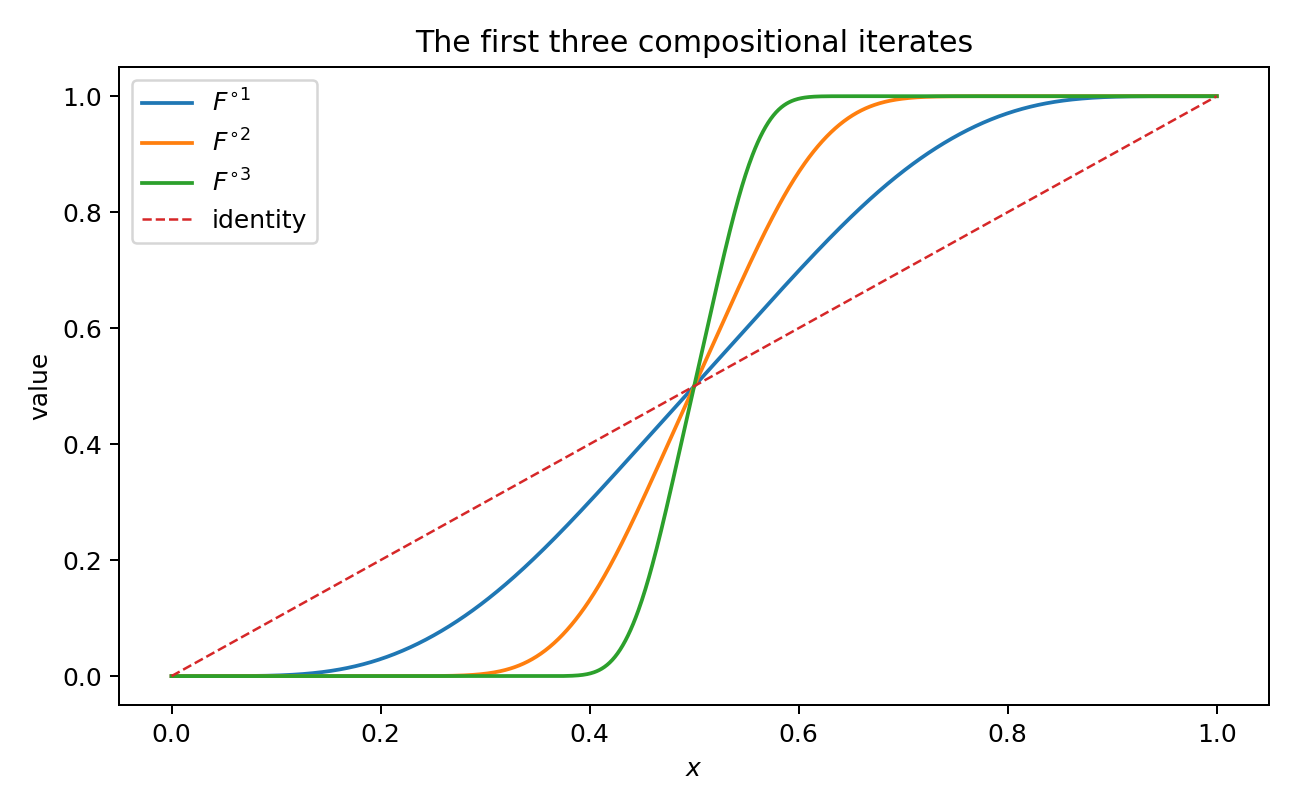
\includegraphics[width=0.86\textwidth]{figures/fabius_iterates.png}
 \caption{Numerical reconstructions of the first three compositional iterates.  The
 strict drift away from the repelling fixed point $1/2$ and toward the endpoints is
 visually apparent.}
 \label{fig:iterates}
\end{figure}

\subsection{Taylor-series composition and the spine comparison}

The default diagnostic point is
\[
 x_0=0.437123456789,
 \qquad n=4.
\]
The computed orbit and prefix weights are
\begin{align*}
 (x_0,x_1,x_2,x_3)
 &\approx(0.4371234568,0.3743185303,0.2522048636,0.07166875375),\\
 (B_0,B_1,B_2,B_3)
 &\approx(1,1.992844087,3.703442407,3.768767090).
\end{align*}
Thus the final orbit level $j=3$ is the unique dominant spine in this example.
Let $D_m$ denote the full numerically composed derivative and $S_m$ the finite spine
sum.  The following table reports both after division by $Q_mH_4^m$, together with
the normalized absolute difference and the $m$-th root of the Taylor coefficient.

\begin{table}[htbp]
\centering
\small
\begin{tabular}{@{}rrrrr@{}}
\toprule
$m$ & $D_m/(Q_mH_4^m)$ & $S_m/(Q_mH_4^m)$
& $\abs{D_m-S_m}/(Q_mH_4^m)$ & $\abs{D_m/m!}^{1/m}$\\
\midrule
10 & $ 1.049415$ & $ 0.721343$ & $3.28\times10^{-1}$ & $ 37.84$\\
12 & $-0.503489$ & $-0.378637$ & $1.25\times10^{-1}$ & $ 60.91$\\
13 & $ 0.961480$ & $ 0.998158$ & $3.67\times10^{-2}$ & $ 84.86$\\
15 & $-0.384836$ & $-0.384202$ & $6.35\times10^{-4}$ & $140.94$\\
16 & $-1.008935$ & $-1.002630$ & $6.31\times10^{-3}$ & $200.75$\\
18 & $ 0.432079$ & $ 0.432434$ & $3.55\times10^{-4}$ & $344.83$\\
19 & $-0.998626$ & $-0.999888$ & $1.26\times10^{-3}$ & $486.69$\\
21 & $ 0.091358$ & $ 0.091354$ & $3.90\times10^{-6}$ & $793.50$\\
22 & $ 0.581063$ & $ 0.581018$ & $4.50\times10^{-5}$ & $1176.18$\\
\bottomrule
\end{tabular}
\caption{Finite-order diagnostic for the spine asymptotic.  Oscillation is expected;
the theorem concerns the normalized absolute remainder, not monotone convergence at
every order.}
\label{tab:numerics}
\end{table}

\begin{figure}[htbp]
 \centering
 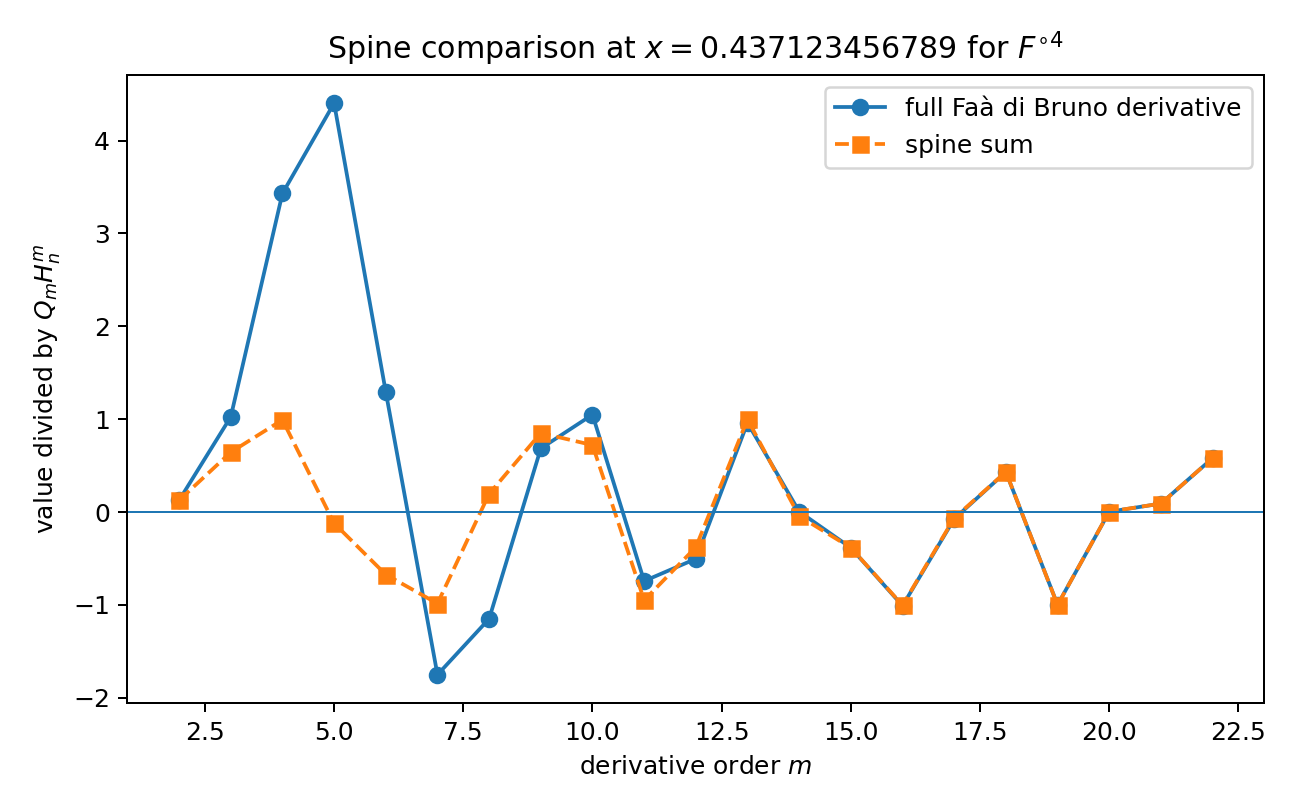
\includegraphics[width=0.86\textwidth]{figures/spine_comparison.png}
 \caption{The full derivative and the finite spine sum after the normalization
 $Q_mH_n^m$.}
 \label{fig:spine-comparison}
\end{figure}

\begin{figure}[htbp]
 \centering
 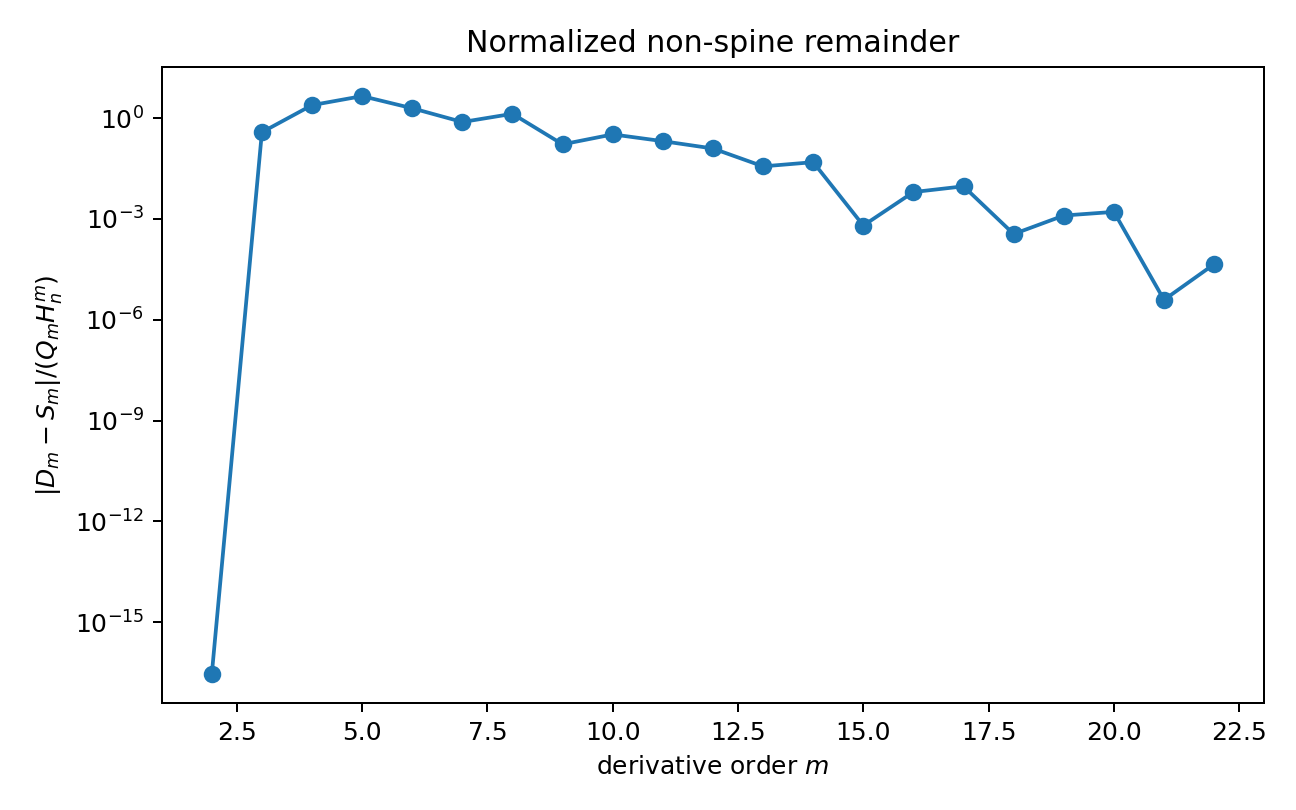
\includegraphics[width=0.86\textwidth]{figures/spine_remainder.png}
 \caption{The normalized non-spine remainder.  Small-order irregularity is compatible
 with the asymptotic statement; the high-order values illustrate the defect-driven
 suppression.}
 \label{fig:spine-remainder}
\end{figure}

The script writes all raw values to \texttt{numerical\_output/}\newline\texttt{spine\_diagnostic.csv},
records orbit metadata, regenerates every figure from command-line parameters,
and synchronizes the four PNG files into the directory read by TeX.
The code contains detailed comments explaining Fourier normalization, the signed
extension, truncated power-series composition, and the spine weights.

\section{Connections to the broader Fabius corpus}
\label{sec:connections}

\subsection{Bell polynomials and Bernoulli cumulants}

Bell polynomials already occur in the repository through moment and cumulant formulae
for dyadic values.  Here the same combinatorial species---set partitions---appears in
a different role: it organizes the derivatives of a composition.  The defect
$D(\pi)$ adds a quadratic dyadic energy to a Bell partition.  This suggests studying
the weighted partition polynomial
\begin{equation}
 \mathcal P_m(z,w)
 :=\sum_{\pi\in\Pi_m}z^{s(\pi)}w^{D(\pi)}.
 \label{eq:defect-polynomial}
\end{equation}
At $w=1$ this collapses toward familiar Bell refinements; at $w=1/2$ it is the exact
suppression factor governing the present proof.  The Bernoulli-cumulant formulas for
$\Up$ arise from logarithms of dyadic products, while \eqref{eq:defect-polynomial}
measures the combinatorics of composing the resulting quadratic-scale jets.  A
$q$-Bell theory with $q=1/2$ may unify these two appearances.

\subsection{q-binomial and Thue--Morse structure}

The exact dyadic values of $F$ are governed by Gaussian-binomial and q-Pochhammer
identities, whereas the derivative signs in \eqref{eq:dyadic-jet} are Thue--Morse.
The present proof shows that under finite self-composition these structures do not
spread across all Fa\`a di Bruno trees at leading order.  They remain concentrated on
a finite set of orbit spines.  The leading sign-amplitude process is
\begin{equation}
 m\longmapsto
 \ThetaF(2^m x_{j_*}),
 \label{eq:leading-symbolic-process}
\end{equation}
which is a direct symbolic sampling of the dyadic shift.  Thus a high-dimensional
Bell expansion asymptotically collapses to a one-dimensional Thue--Morse-modulated
orbit observable.

\subsection{Infinite sinc products}

The sinc product \eqref{eq:sinc-product} supplies the numerical representation used
here and explains the exceptional smoothness of $\Up$.  The nowhere-analyticity
mechanism, however, is most transparent in physical space: dilation creates $Q_m$,
block translation creates Thue--Morse signs, and binary transitions prevent the
amplitude from becoming too small forever.  The Fourier and derivative pictures are
therefore complementary.  A possible future goal is to derive the spine expansion
directly from a multidimensional Fourier integral for $F^{\comp n}$, but nonlinear
composition makes such a representation substantially less direct than the
set-partition proof.

\subsection[Lambert-W endpoint asymptotics]{Lambert--$W$ endpoint asymptotics}

The repository develops small-argument asymptotics of $F$ in which lower real branches
of the Lambert--$W$ function encode the saddle point.  For a fixed $n$, the left-half
dynamics repeatedly applies an extremely flat map:
\begin{equation}
 x\mapsto F(x)\mapsto F(F(x))\mapsto\cdots.
 \label{eq:nested-flat-map}
\end{equation}
The present derivative theorem is local in the differentiation order $m$, while the
Lambert--$W$ theory is local in $x\downarrow0$.  Their intersection is a two-parameter
problem: asymptotics of $G_n^{(m)}(x)$ when both $m\to\infty$ and $x\downarrow0$.
The spine formula predicts phase transitions when the maximizing prefix $B_j$ changes
orbit level.  Those transition surfaces are natural candidates for nested
Lambert--$W$ descriptions.

\subsection{Legendre expansions and polynomial representations}

The Rvachev function admits rapidly convergent orthogonal-polynomial expansions, and
the repository investigates representations of polynomials by shifted $\Up$ copies.
Since $G_n$ becomes increasingly step-like around $1/2$ as $n$ grows, its Legendre
coefficients should exhibit a two-scale pattern: smooth compact-kernel decay at fixed
$n$, followed by a singular limit as $n\to\infty$.  Theorem \ref{thm:main} forbids
exponential coefficient decay strong enough to imply analyticity in a Bernstein
ellipse touching any real subinterval.  Quantifying the exact subexponential decay
would connect the present local derivative obstruction to global approximation theory.

\section{Conjectures and research directions}
\label{sec:future}

The theorem settles nowhere analyticity, but the exceptional countable set left by the
proof contains interesting arithmetic structure rather than a genuine gap in the main
conclusion.

A tempting strengthening would assert zero Taylor radius at every interior point.
That statement is already false for $n=1$: at a dyadic point, the high-order jet of
$F$ eventually vanishes, so the formal Taylor series is a finite polynomial, although
it does not represent $F$ on any neighborhood.  The appropriate open problem is a
classification rather than a universal zero-radius assertion.

\begin{warning}[Quarantined Taylor-series trichotomy]
\label{warn:trichotomy-quarantine}
The former conjecture proposed that, for fixed $n$, every interior point belongs
to exactly one of three explicitly classifiable classes:
\begin{enumerate}[label=(\roman*)]
 \item the Taylor series has radius zero;
 \item the Taylor series is a finite polynomial because the entire high-order jet
 eventually vanishes;
 \item the Taylor series has positive radius but does not represent the function.
\end{enumerate}
This is not an exclusive trichotomy as written.  At an interior dyadic point for
$n=1$, the eventually zero jet gives a finite polynomial Taylor series; that series
also has positive radius and does not represent $F$ on a neighborhood.  Such a point
therefore satisfies both (ii) and (iii).  Any repaired classification must explicitly
exclude eventually zero series from (iii).  The detailed classification for $n\geq2$
remains an open problem, but no corrected conjecture is asserted here.
\end{warning}

This quarantine illustrates why it is valuable to distinguish nowhere
analyticity from zero Taylor radius.  The present theorem proves class (i) on a
co-countable set and rules out local representation everywhere, while the detailed
Taylor behavior at the exceptional points remains open for $n\geq2$.

\begin{warning}[Quarantined tie-cancellation conjecture]
\label{warn:ties-quarantine}
The former conjecture asserted that, when $x\in T_n$ and two adjacent spine
weights are maximal, their two leading terms cannot cancel to exponential accuracy
at every sufficiently large order.  It is not retained as an open conjecture.  The
canonical quarter-point identities $F'(1/4)=F'(3/4)=1$, together with the strict
slope monotonicity used above, show that the tied orbit point $x_k$ is $1/4$ or
$3/4$.  Hence $\ThetaF(2^m x_k)=0$ for $m\geq3$.  The next orbit point is
$x_{k+1}=5/72$ or $67/72$, respectively, and is not dyadic.  By
\cref{lem:binary-transition}, along infinitely many orders its amplitude has
absolute value at least $1/2$.  On that subsequence the first tied term vanishes and
the second has absolute value at least
$A_{k+1,n}H_n(x)^m/2$, which is the proposed conclusion with a positive constant.
This deduction remains at manuscript level because the $n\geq2$ spine expansion is
not yet formalized in Lean.
\end{warning}

\begin{conjecture}[Defect-polynomial spectral gap]
\label{conj:defect-polynomial}
For every fixed $z>0$, the weighted partition sums
\[
 \sum_{\substack{\pi\in\Pi_m\\1<|\pi|<m}}z^{s(\pi)}2^{-D(\pi)}
\]
admit a full asymptotic expansion whose leading term comes from partitions with one
block of size $2$ and all remaining blocks singleton, together with the dual family
of one block of size $m-1$ and one singleton.
\end{conjecture}

The proof of \cref{prop:defect-decay} is deliberately coarse.  Sharp asymptotics would
produce an explicit rate in the spine theorem and might support uniform estimates in
$x$ away from orbit tie surfaces.

\subsection{Promising formalization route}

A Lean formalization can be modular.
\begin{enumerate}[label=\arabic*.]
 \item Define $Q_m$ and prove the algebraic identity
 \eqref{eq:Q-factorization} for finite set partitions.
 \item Formalize the two extremal partitions and the defect-zero classification.
 \item Replace the asymptotic counting proof initially by a stronger but simpler
 explicit estimate sufficient for $\littleo(1)$.
 \item Use the existing iterated-derivative and bounded-derivative APIs for $F$.
 \item Prove the spine expansion by induction on the fixed iterate count.
 \item Reuse the existing strict monotonicity, convexity, order-isomorphism, and
 Thue--Morse modules to construct $E_n$ and the dominant subsequence.
 \item Finish with the existing analytic-at and power-series-radius infrastructure.
\end{enumerate}
The combinatorial proposition is the only substantial library-building step.  Once it
is available, the analytical induction closely follows the existing module style.

\subsection{Generalization to other atomic functions}

The proof abstracts beyond the classical dyadic Fabius function.  Suppose a smooth
map $f$ has derivatives
\begin{equation}
 f^{(m)}(x)=q^{\binom{m+1}{2}}\Phi(q^m x)
 \label{eq:q-atomic-derivatives}
\end{equation}
for some $q>1$, with bounded $\Phi$, recurrent nonvanishing along a dense set of
$q$-adic orbits, and monotone orbit slopes that yield a unique dominant prefix.
The same defect calculation works with $2^{-D(\pi)}$ replaced by $q^{-D(\pi)}$.
This suggests a general theorem for Rvachev-type atomic functions beyond the dyadic
case, including multiscale refinable functions with a one-branch derivative law.

\section{Summary of the proof mechanism}

For reference, the entire argument can be compressed into the following chain.
\begin{enumerate}[label=\arabic*.]
 \item Exact differentiation gives $F^{(m)}=Q_m\ThetaF\comp(2^m\cdot)$ with
 $Q_m=2^{m(m+1)/2}$ and $\abs\ThetaF\leq1$.
 \item In Fa\`a di Bruno's set-partition formula, every non-spine partition has a
 positive quadratic defect $D(\pi)$.
 \item The weighted sum of all non-spine partitions is exponentially small, despite
 the Bell-number multiplicity.
 \item Therefore $G_n^{(m)}$ is asymptotic, after division by $Q_m$, to a finite sum
 of orbit spines $A_{j,n}B_j^m\ThetaF(2^m x_j)$.
 \item Away from a finite tie set, monotone orbit dynamics makes one $B_j$ uniquely
 maximal.
 \item Away from countably many dyadic orbit preimages, binary digit transitions make
 the dominant amplitude at least $1/2$ infinitely often.
 \item Hence $\abs{G_n^{(m)}(x)}\geq cQ_mH_n^m$ infinitely often on a co-countable
 dense set.
 \item Since $Q_m^{1/m}/(m!)^{1/m}\geq2^{(m+1)/2}/m\to\infty$, the Taylor radius is
 zero there.
 \item Analyticity at any point would imply analyticity on a neighborhood containing
 one of those dense zero-radius points, a contradiction.
\end{enumerate}

\appendix

\section{Auxiliary details on the partition defect}
\label{app:defect}

This appendix records two identities useful for sharpening
\cref{prop:defect-decay}.

\begin{proposition}[Exact minimum at fixed block count]
\label{prop:fixed-k-minimum}
Among partitions of $m$ with $k$ blocks,
\begin{equation}
 \min D(\pi)=(k-1)(m-k).
 \label{eq:fixed-k-minimum}
\end{equation}
Equality holds exactly when one block has size $m-k+1$ and every other block is a
singleton.
\end{proposition}

\begin{proof}
For fixed $m,k$, formula \eqref{eq:defect} shows that minimizing $D$ is equivalent to
maximizing $\sum_i\binom{r_i}{2}$.  Strict convexity of $r\mapsto\binom r2$ transfers
one unit from a smaller nonsingleton block to a larger block and increases the sum.
Iteration leaves one large block and $k-1$ singletons.  Direct substitution gives
\eqref{eq:fixed-k-minimum}.
\end{proof}

\begin{proposition}[First defect shell]
\label{prop:first-shell}
For $m\geq3$, the least positive defect is $m-2$.  It occurs for exactly two block-size
profiles:
\begin{equation}
 (2,1,\ldots,1)
 \qquad\text{and}\qquad
 (m-1,1).
 \label{eq:first-shell}
\end{equation}
\end{proposition}

\begin{proof}
From \eqref{eq:fixed-k-minimum}, the least positive value over $2\leq k\leq m-1$ is
\[
 \min_{2\leq k\leq m-1}(k-1)(m-k)=m-2,
\]
attained only at $k=2$ and $k=m-1$.  The equality classification in
\cref{prop:fixed-k-minimum} gives the two profiles.
\end{proof}

This identifies the candidate leading correction to the spine sum.  At the
near-singleton end, choose one pair and leave all other elements singleton; at the
near-giant end, choose the singleton outside a block of size $m-1$.  Both carry the
same dyadic penalty $2^{-(m-2)}$, but their derivative coefficients and orbit factors
are different.  A refined expansion should sum these shells before estimating the
higher-defect remainder.

\section{Reproducibility guide}
\label{app:reproducibility}

The archive contains the following files.
\begin{longtable}{@{}p{0.40\textwidth}p{0.52\textwidth}@{}}
\toprule
File & Purpose\\
\midrule
\endhead
\texttt{fabius\_iterates\_nowhere\_}\newline\texttt{analytic.tex}
& Complete LaTeX source of this report.\\
\texttt{fabius\_iterates\_nowhere\_}\newline\texttt{analytic.pdf}
& Rendered report.\\
\path{numerical_experiments.py}
& Commented Python program for sinc-product reconstruction, Taylor composition,
spine evaluation, CSV output, and figures.\\
\texttt{numerical\_output/}\newline\texttt{spine\_diagnostic.csv}
& Raw derivative and spine diagnostics through the selected maximum order.\\
\texttt{numerical\_output/}\newline\texttt{numerical\_metadata.txt}
& Parameters, orbit points, slopes, prefixes, suffixes, and dominant weight.\\
\path{figures/*.png}
& Synchronized figure copies: three are included in the report and the Taylor-root
diagnostic is retained as supplementary output.\\
\bottomrule
\end{longtable}

A typical reproduction command is
\begin{lstlisting}[style=pseudo,language=bash]
MPLBACKEND=Agg python numerical_experiments.py \
  --output-dir numerical_output \
  --figure-dir figures \
  --x0 0.437123456789 \
  --iterate-count 4 \
  --max-order 22
\end{lstlisting}
The program requires Python 3, NumPy, SciPy, and Matplotlib.  It records values at
$\Up(0)$, $\Up(1/2)$, $F(0)$, $F(1/2)$, and $F(1)$ before writing output, while
enforcing numerical tolerances only at $\Up(0)$ and $F(1/2)$.  Exact PNG bytes and
the final floating-point digits depend on the pinned platform and dependency stack
recorded in the repository audit; the CSV record terminator is fixed explicitly to LF.

\section{Repository source map}
\label{app:source-map}

Under the common root \path{Analysis/FabiusFunction/}, the repository paths most
directly connected to the proof are:
\begin{itemize}[leftmargin=2em]
 \item \path{docs/Fabius_Function_and_Rvachev_Up/}
 for the primary exposition;
 \item \path{GlobalExtension.lean}
 and \path{BoundedDerivatives.lean} in \path{Lean/FabiusFunction/} for the derivative atlas;
 \item \path{Convexity.lean}, \path{Monotonicity.lean}, and the order-isomorphism
 modules for the orbit dynamics;
 \item \path{OriginalPaperSupplement.lean} and \path{NowhereAnalytic.lean} for the
 base nonanalyticity proof;
 \item \path{docs/Non_Elementarity_of_the_Fabius_Function/} for the dense
 analytic-locus obstruction;
 \item \path{docs/semi-formalized-research-frontiers/} for q-series, Bell/Bernoulli,
 sinc-product, Lambert--$W$, Legendre, and other frontier connections;
 \item \path{docs/archive/} and the frontier README for provenance and consolidation
 of historical TeX drafts.
\end{itemize}

\small
\begin{thebibliography}{99}

\bibitem{Fabius1966}
J.~Fabius,
\newblock A probabilistic example of a nowhere analytic $C^\infty$-function,
\newblock \emph{Z. Wahrscheinlichkeitstheorie verw. Geb.} \textbf{5} (1966),
173--174.

\bibitem{Arias1982}
J.~Arias de Reyna,
\newblock An infinitely differentiable function with compact support: definition and
properties,
\newblock English translation of \emph{Rev. Real Acad. Ciencias Madrid} \textbf{76}
(1982), 21--38, arXiv:1702.05442.

\bibitem{AriasArithmetic}
J.~Arias de Reyna,
\newblock Arithmetic of the Fabius function,
\newblock arXiv:1702.06487v3, 2017.

\bibitem{Comtet}
L.~Comtet,
\newblock \emph{Advanced Combinatorics: The Art of Finite and Infinite Expansions},
\newblock revised and enlarged edition, D. Reidel, 1974.

\bibitem{Johnson2002}
W.~P. Johnson,
\newblock The curious history of Fa\`a di Bruno's formula,
\newblock \emph{American Mathematical Monthly} \textbf{109} (2002), 217--234.

\bibitem{KrantzParks}
S.~G. Krantz and H.~R. Parks,
\newblock \emph{A Primer of Real Analytic Functions},
\newblock second edition, Birkh\"auser, 2002.

\bibitem{ProveItPrimary}
V.~Reshetnikov,
\newblock \emph{The Fabius Function and Rvachev's Up Function},
\newblock proof-backed primary exposition in the ProveIt repository,
\newblock \url{https://github.com/VladimirReshetnikov/ProveIt/tree/main/Analysis/FabiusFunction},
accessed 30 August 2026.

\bibitem{ProveItFrontier}
V.~Reshetnikov,
\newblock \emph{Semi-formalized Research Frontiers for the Fabius Function},
\newblock canonical frontier synthesis in the ProveIt repository, accessed
30 August 2026.

\end{thebibliography}

\end{document}
